\graphicspath{{chapters/detector/images/}}
\chapter{The IceCube Detector}
\label{chapter:detector}
There exist two avenues for the measurement of neutrinos.
The precise measurements of individual events, used most notably in the OPERA \cite{Description-OPERA} and DONUT \cite{DONUT-2001} experiments to identify individual events, gives unique constraining power with low backgrounds.
More common, however, is the use of large experimental volumes to collect high-statistics neutrino samples.
For the study of atmospheric neutrinos, volumes on the order of a kiloton are required. 

The IceCube Neutrino Observatory is currently the largest neutrino detector in the world, encompassing a volume of 1 km$^3$ of glacial ice at the geographic south pole.
The design of the IceCube detector is also presented in this chapter, beginning with a description of the DOMs that make up the primary detectors within the IceCube observatory (Section~\ref{sec:dom}).
The overall geometry of the detector is discussed in Section~\ref{sec:geometry} with a focus on the differences between the larger IceCube detector and the DeepCore subarray used for oscilation searches.

\section{The DOM: The Basic Unit of IceCube}
\label{sec:dom}

The basic unit of the IceCube detector is the \emph{digital optical module}, often referred to simply as the \emph{DOM} \cite{Description-IceCube}.
The DOM is designed around a downward-facing 10 inch R7081-02 photomultiplier tube (\emph{PMT}) from Hammamatsu Photonics \cite{IceCube-PMT,IceCube-PMT-Hammamatsu} and includes onboard electronics for standard operation as shown in Figure~\ref{fig:icecube_dom}. 
Circuit boards are included for data acquisition, control, calibration, communications and power conversion as well as for high voltage input from the surface.
The electronics of the DOM are encased in a spherical glass housing designed to withstand the high pressures associated with operation in the glacier of Antarctica.

The IceCube PMTs are used to detect Cherenkov photons produced by particle interactions in the ice.
The PMT of an IceCube DOM sensitive to wavelengths between 300 nm and 650 nm with a peak quantum efficiency of about 25\% for standard PMTs \cite{Description-IceCube}.
The PMT is optically coupled to a glass pressure housing enclosing the DOM to minimize distortion of incoming light.

\begin{figure}
\centering
\includegraphics[width=0.4\textwidth]{icecube_dom.png}
\caption[The IceCube DOM]{The IceCube DOM contains multiple components, including the PMT itself, onboard calibration devices, and various electronics necessary for semi-autonomous operation.}
\label{fig:icecube_dom}
\end{figure}

\label{subsubsec:pulsing}
\subsubsection{Pre-, Late-, and Afterpulsing}
A PMT amplifies signals of electrons emitted from a photocathode due to incident light, producing a voltage drop at the anode called a \emph{pulse}.
Errors in the amplification process can introduce additional pulses reaching the anode.
These effects are divided into \emph{pre-pulses}, \emph{late-pulses}, and \emph{afterpulses}.

\begin{figure}
\centering
\includegraphics[width=0.4\textwidth]{afterpulsing.png} 
\caption[Afterpulsing calibrations in IceCube]{Afterpulsing calibration measurements performed in the lab. LEDs with known brightness were flashed to test for off–time response of the IceCube PMT. Clear dips, corresponding to detected charge, are visible. Drop (a) corresponds to the initial LED flash while (b), (c), and (d) show prominant afterpulsing peaks. Image taken from \cite{IceCube-PMT}.}
\end{figure}
The pre-pulses, arriving within a few dozens of nanoseconds prior to the main pulse, arise from the small probability of an electron bypassing one of the dynodes. 
Late-pulses are likewise thought to be produced by electrons which return to a previous dynode, inducing a signal a few dozens of nanoseconds immediately following the main signal.
These signals tend to be small and inconsequential for physics measurements.

Afterpulses are produced from ionization of residual gases in the PMT.
The ionized atoms tend to travel significantly more slowly than electrons, resulting in a delay between the main signal and the subsequent afterpulses that may be as large as 10 microseconds.
The afterpulses require dedicated calibration and mismodeling may affect other measurements as addressed in Section~\ref{sec:vuvuzela_limitations}.

\subsection{The Discriminator Used for DOM Triggering}
\label{ubsec:discriminator}
A discriminator onboard the DOM is used to identify signals from the PMT with a voltage threshold corresponding to 0.25 photoelectrons (\emph{PE}).
Each discriminator crossing begins a \emph{DOM launch}, the lowest level signal available in the IceCube detector containing a digitized representation of the raw PMT output in the form of a \emph{waveform}.
Launches are stored in DOM memory while awaiting a decision from the triggering system.

\subsection{Local Coincidence}
\label{subsec:LC}
If any of the notified DOMs also record a launch within a configurable 1 microsecond window, both launches are said to form a \emph{hard local coincidence} (\emph{HLC}) pair.
Nearby DOMs, here defined to be either of the two DOMs above or below the current DOM, are notified of the launch via a signal sent using the \emph{local coincidence} wiring.
Launches which fail to satisfy the local coincidence conditions are referred to as \emph{soft local coincidence} (\emph{SLC}) launches.
Launches recorded as part of an HLC pair receive a flag to record local coincidence status.
This flag may be used to later identify only those launches which satisfy the local coincident conditions, providing a simple, default method of identifying hits likely to be caused by particle interactions in the detector.

\subsection{Digitization}
\label{subsec:digitization}
While awaiting a local coincidence decision, the waveform of a launching DOM is passed to the two onboard digitizers.
Information from the PMT is digitized using the fast analog-to-digital converter (\emph{FADC}), which provides binned information at 40$\times 10^6$ samples/second for the 6.4 microseconds following the initial DOM launch \cite{Description-IceCube}.
Simultaneously, the \emph{Analog to Digital Waveform Digitizer}, or \emph{ATWD}, will digitize the waveform using 322 bins with 3.3 nanoseconds per bin. 

If a launch satisfies the HLC conditions, the DOM will request the full digitization of the waveforms from both the ATWD and FADC, providing a complete record of the launch.
Examples of digitized waveforms from the ATWD and fADC are shown in Figure~\ref{fig:waveforms}.

When digitizing a signal, the ATWD experiences up to 29 microseconds of deadtime \cite{Description-IceCube}. 
During this time, the secondary ATWD is available to record further pulses, resulting in a total average fractional deadtime per DOM of ${2.2 \times 10^{-5}}$ seconds/second.
In addition, each of the two ATWDs possesses three channels with separate gains.
This provides the ability to accurately measure the waveform, even in cases of saturation of high gain channels.
The unsaturated ATWD with the highest gain provides a record for the launch.

If the launch fails the HLC launch criteria, the information in the ATWD ceases the digitization process and the FADC instead digitizes only the three bins associated with the largest peak of the waveform.
While this limits the information available for these launches, the lack of associated nearby launching DOMs provides strong evidence that the launch is due to random detector noise.

\begin{figure}
\centering
\includegraphics[width=0.6\textwidth]{icecube_waveforms.png}
\caption[Examples of IceCube digitized waveforms]{Examples of the ATWD (top) and FADC (bottom) waveforms output from an IceCube PMT. Taken from \cite{Description-IceCube}}
\label{fig:waveforms}
\end{figure}

\subsection{Noise in IceCube DOMS}
\label{subsec:noise}
Dedicated measurements using IceCube DOMs have shown multiple components to the detector noise\cite{Thesis-Vuvuzela}. 
A large fraction of the detector noise displays non-Poissonian behavior in time \cite{Description-IceCube}.
The model used in IceCube, shown in Figure~\ref{fig:noise_model}, splits the detector noise into \emph{Poissonian} and \emph{non-Poissonian}(\emph{time-correlated}) noise.

\begin{figure}
\centering
\includegraphics[width=0.6\textwidth]{vuvuzela.png} 
\caption[The timing structure of noise in the IceCube detector]{A histogram of the time between subsequent hits on DOM 15 of string 27. Hitspool data, specialized data collected with no trigger applied, is shown in blue. The "correlated" (non-Poissonian) and "uncorrelated" (Poissonian) features are shown in red and black respectively. The location of a large afterpulsing peak is shown in yellow. Note that the features included are not to scale. Image taken from \cite{Description-IceCube}.}
\label{fig:noise_model}.
\end{figure}

The Poissonian noise consists of thermal noise and radiactive decays in the glass of the PMT and DOM.
Studies of these radioactive components are ongoing, with some evidence that Potassium-40 and Uranium-238 may be responsible for at least some of the observed decays.
Once a decay occurs, a rapid series of pulses occurs in the PMT, leading to a "burst" of noise that continues for up to a few milliseconds \cite{Thesis-Vuvuzela}. 
These hits are believed to be due to a scintillation or luminescence process.

The typical averaged noise rate is 560 Hz for standard IceCube DOMs and 780 Hz for high quantum efficiency DOMs.
Poissonian noise makes up approximately 250 Hz of this rate with the remainder due to non-Poissonian processes.

\subsection{Triggering in IceCube}
\label{subsec:triggers}
Digitized versions of the waveforms are transmitted from the DOM to the IceCube physics data acquisition system (\emph{pDAQ}) for use in trigger and event building.
The most common type of trigger used in IceCube analyses is the \emph{Simple Majority Trigger} or \emph{SMT}. 
This trigger is designed to look for coincidences between DOMs using HLC launches.
Each of the SMTs is defined by three fundamental configurations: a DOMSet, which lists the DOMs available for use in the trigger conditions; a threshold number of HLC launches before the trigger fires; and a time window length, $\Delta t_{trig}$ in which the HLC are required to coexist.
The trigger time, $t_{trig}$ is defined to be the time of the first contributing HLC launch.

Information from the detector is recorded in a \emph{readout window} around each trigger from $t_{trig} - 4 \mu s$ to $t_{trig} + \Delta t_{trig} + 6 \mu s$ around each trigger time.
Once all triggers are identified, a \emph{global trigger} is defined as the union of all overlapping readout windows.




\section{Pulse Extraction}
\label{sec:wavedeform}
The extraction of charge and timing information from recorded waveforms is performed using the \emph{wavedeform} module, which accepts and processes the information from the launches in each triggered event.
Wavedeform reconstructs the original charge information from the digitized waveform information.

Wavedeform uses a parametrized version of the PMT pulse associated with a single photoelectron describing the timing and charge profile of the PMT amplification process. 
Beginning with a single pulse template, a least squares minimization is performed to find the best-fit time of a single pulse in the observed waveform.
Additional copies of the pulse template are added and new minimizations are performed until the goodness-of-fit improvement from additional pulses is negligible.
The resulting sets of pulses, including associated timing and normalization, are returned as \emph{reconstructed pulses}, often referred to more informally as either \emph{pulses} or \emph{hits}.
These pulses represent the best-fit recreation of the analog pulses in the PMT prior to the digitization process.

Both HLC and SLC waveforms are fit, although the limited information in SLC waveforms necessarily results in the loss of information.
Information from the ATWD is preferred over information from the FADC for pulse extraction of HLC waveforms.




\section{The Geometry of the Detector}
\label{sec:geometry}
The IceCube detector is located at the geographic south pole in Antarctica.
The Antarctic glacier forms a 2.8~km deep surface of clear ice over the bedrock.
IceCube uses the Antarctic glacier as both a support structure and as a detection medium for Cherenkov radiation.

\begin{figure}
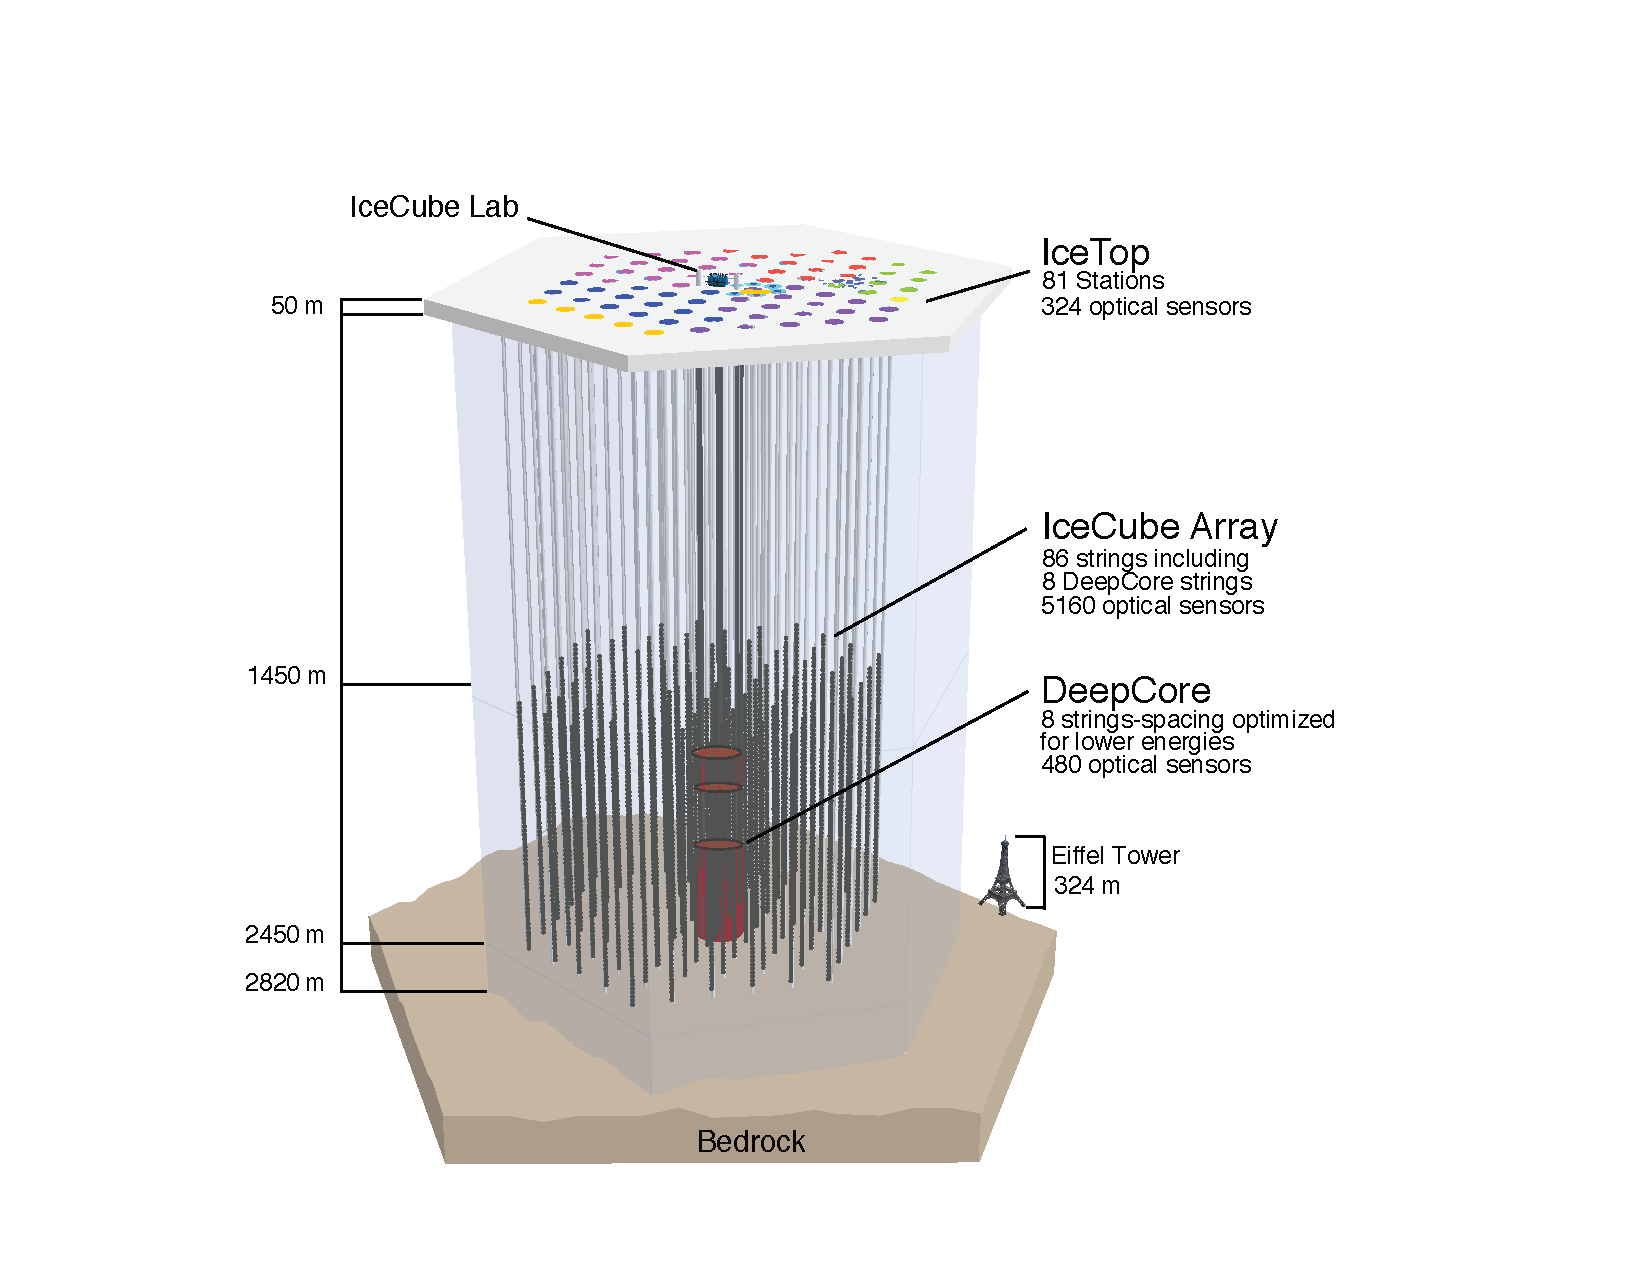
\includegraphics[width=0.9\linewidth]{ArrayWSeasonsLabels.pdf}
\caption[An overview of the subdetectors in the IceCube Neutrino Observatory]{The IceCube Neutrino Observatory. Three separate subdetectors are shown: IceTop, a cosmic ray air shower detector; IceCube, an array designed to search for astrophysical neutrinos; and DeepCore, a dense subarray used for atmospheric oscillation physics measurements. The detector was deployed over multiple years. Strings deployed in the same year are shown with identical colors at the surface. }
\label{fig:icecube_depth}
\end{figure}

The IceCube observatory consists of three distinct subarrays, shown in Figure~\ref{fig:icecube_depth}, each optimized for separate physics measurements.
A total of 5160 DOMs make up the IceCube in-ice array with an additional 324 DOMs used at the surface in the IceTop air shower array \cite{Description-IceCube}.
IceCube DOMs are deployed at depths between 1450~m and 2450~m below the surface to shield the detector from atmospheric background muons.
The DOMs are deployed in a hexagonal grid in a series of 86 vertical \emph{strings}, each of which provides connections and support for 60 DOMs.
Strings are spaced approximately 125~m apart with DOMs space 17~m apart on each string.
Each DOM in the IceCube detector is assigned a unique string number (1-86) and DOM number (1-60).

\begin{figure}
\centering
\includegraphics[width=0.6\textwidth]{dc_layout.pdf} 
\caption[The IceCube and DeepCore string geometry]{The layout of the IceCube and DeepCore detectors. DeepCore is installed at the bottom of the IceCube detector in the clearest ice. A subset of DOMs were also deployed above DeepCore to improve muon identification of very-downgoing events.}
\label{fig:deepcore_layout}
\end{figure}

Strings were installed in the glacier annually from 2004 until 2010 with partial detector data collected during construction.
During the final years of construction, a denser section of the detector was built, known as DeepCore \cite{Description-DeepCore}.
The DeepCore subarray consists of 8 strings equiped with high quantum efficiency PMTs 34\% more sensitive than the standard IceCube PMT \cite{IceCube-PMT}.
The DeepCore strings are split between a \emph{fiducial} volume, in which 50 DOMs are spaced 7~m apart on a string, and a \emph{veto plug} of 10 DOMS 10~m apart as shown in Figure~\ref{fig:deepcore_layout}.
The DOMs in the DeepCore fiducial volume are located in the clearest ice of the detector at depths between 2100~m and 2450~m below the surface \cite{IceCube-SpiceMie}.
The veto cap, installed between 1750 and 1850~m below the surface, is used to identify background muons for DeepCore.

\subsection{IceCube: A Detector for TeV Neutrinos}
\label{subsec:icecube}
The IceCube detector is a regularly spaced hexagonal grid buried in the glacier with the purpose of measuring astrophysical neutrinos and identify the source of cosmic rays.
The IceCube array has an energy threshold of around 50-100~GeV with an optimal response above 1~TeV \cite{Description-DeepCore, Description-IceCube}.

In the standard IceCube detector, an SMT using all DOMs with a threshold of 8 HLC launches within a 5 microsecond trigger time window \cite{Description-IceCube}.
This trigger, known as \emph{SMT8} after the number of required launches, is designed for high signal efficiency at energies above 100~GeV with a minimum number of accidental triggers due to detector noise.
The IceCube detector records an SMT8 rate of around 2100~Hz with less than 1~Hz expected from neutrino interactions and the remainder primarily due to muons produced in cosmic ray showers in the Earth's atmosphere.

Events at the TeV scales of the IceCube detector show well-defined topologies, as shown in Figure~\ref{fig:icecube_he_events}.
The IceCube detector has performed many measurements, including searches for sterile neutrinos \cite{IceCubeSterile-IC86-1}, anisotropy in the cosmic ray flux \cite{IceCube-CRAnisotropy}, measurements of the neutrino cross section at high energies \cite{IceCube-Xsec}, and the discoveries of an astrophysical neutrino flux \cite{IceCube-HESE6}.

\begin{figure}[h]
\centering
\begin{tabular}[b]{c}
  \includegraphics[width=0.3\linewidth]{icecube_he_nue.png} \\
  \small (\textbf{\color{ctcolormain}a}) $\nu_e$ CC, $\nu$ NC
\end{tabular} \hspace{2pt}
\begin{tabular}[b]{c}
  \includegraphics[width=0.3\linewidth]{icecube_he_numu.png} \\
  \small (\textbf{\color{ctcolormain}b}) $\nu_\mu$ CC
\end{tabular}
\begin{tabular}[b]{c}
  \includegraphics[width=0.3\linewidth]{icecube_he_nutau.png} \\
  \small (\textbf{\color{ctcolormain}c}) $\nu_\tau$ CC]
\end{tabular}
\caption[Event signatures above 1~TeV in IceCube]{Examples of event signatures above 1~TeV using the full IceCube array. Event views shown in (a) and (b) are from actual events discovered by IceCube \cite{IceCube-AstroNu}. Images taken from \cite{Thesis-Euler}. (a)$\nu_e$ CC and $\nu$ NC show similar behavior from electromagnetic and hadronic interactions, which result in a shower of particles that quickly scatter in the ice. Cherenkov emission from these events appears roughly spherical in the detector. These events are known as "cascades". (b) $\nu_\mu$ CC events begin with a hadronic interaction, then produce Cherenkov light from the outgoing muon. The track of the outgoing muon is clearly visible. (c) Above 1~PeV, the tau lepton from a $\nu_\tau$ CC interaction may travel a significant distance before decaying. This results in two well-separated cascades in the detector, a tell-tale signature of $\nu_\tau$ CC interactions. Tau neutrino interactions below 1~TeV are not distinguishable from  other cascade-like events.}
\label{fig:icecube_he_events}
\end{figure}

\subsection{DeepCore: Extending the Reach to~GeV Scales}
\label{subsec:deepcore}
The DeepCore detector was designed to be a smaller, denser detector used in the study of GeV neutrinos.
The denser spacing and clear ice of DeepCore lowers the energy threshold to around 10~GeV from IceCube's threshold of around 100 GeV \cite{Description-DeepCore}, permitting the study of oscillations.


In DeepCore, the desire for lower energy events led to the introduction of a separate trigger, known as \emph{SMT3}.
This trigger, using only DOMs within the DeepCore fiducial volume, searches for at least three HLC launches occuring within 2.5 microseconds.
This effectively lowers the triggering threshold from roughly 100~GeV with the larger IceCube array to approximately 10 GeV.
The SMT3 rate, at 250 Hz \cite{Description-IceCube, Description-DeepCore}, is substantially smaller than the SMT8 rate due to both the increased overburden as well as the smaller number of PMTs included in the SMT3 DOMSet.
By placing the detector inside of the larger IceCube array, DeepCore allows analyzers to use the IceCube detector as an active veto, reducing the background rate to 17 Hz.

DeepCore events do not show the clean topological separation of the higher energy IceCube events as seen in Figure~\ref{fig:icecube_he_events}.
Events may be separated broadly into \emph{cascade-like} and \emph{track-like} statistically using information contained in the timing of hits in the detector.
Such separation techniques are energy-dependent and do not perform well at very low energies.

\begin{figure}
\centering
\includegraphics[width=0.9\linewidth]{deepcore_le_views.png} 
\caption[Event topologies of 50~GeV events in DeepCore]{A selection of 50~GeV simulated events in DeepCore taken from \cite{Thesis-Euler}. Unlike the event topologies at high energies, DeepCore events do not show distinct event types.}
\label{fig:deepcore_events}
\end{figure}

DeepCore has observed atmospheric neutrino oscillations in the $\nu_\mu \rightarrow \nu_\tau$ in the disappearance channel \cite{IceCube-Oscillation2013,IceCube-Oscillation2015,IceCube-Oscillation2018}, with the most recent measurement showing competitive precision to dedicated measurements performed with particle accelerators.

While DeepCore was designed for oscillation physics, the neutrinos may be used for other purposes as well. 
Recent work with DeepCore has shown sensitivity to studying dark matter interactions in the sun \cite{IceCube-LE-SolarDarkMatter} and in the galaxy \cite{IceCube-LE-GalacticDarkMatter}.









\section{The Bulk Ice Model}
\label{sec:bulk_ice}
The Antarctic glacier, with a thickness of 2.8~km at the geographic south pole \cite{IceCube-SpiceMie}, forms both the support structure and the interaction medium for IceCube.
Measurements of the dust concentration of the ice as a function of depth were taken during deployment of the IceCube strings.
The IceCube dust logger emitted laser light aimed into the undrilled ice and detected backscattered photons\cite{IceCube-DustLogger1, IceCube-DustLogger2}.
The results are shown in Figure~\ref{fig:dust_logger}.

\begin{figure}[h]
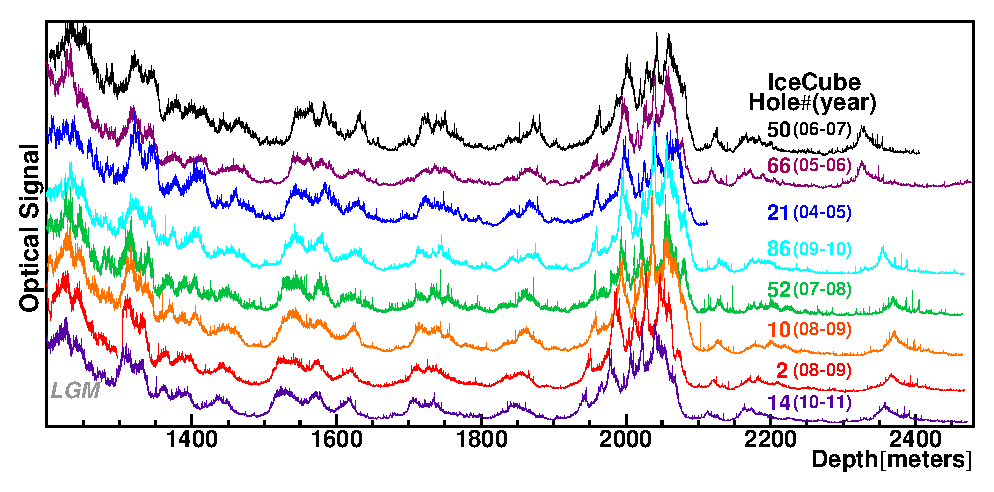
\includegraphics[width=0.9\textwidth]{dustlogger.eps} 
\caption[Dust concentration measurements from deployment of strings]{The data from the dust loggers deployed in various drill holes in IceCube during deployment. Data from individual holes has been offset in the y direction for clarity. Larger relative values of the "Optical Signal" represent more scattering in the ice while smaller values indicate clearer ice. The "dust layer" is visible in all drill holes around 2000 m. Deepcore DOMs are deployed below this layer. Image taken from \cite{IceCube-DustLogger-Raw}.}
\label{fig:dust_logger}
\end{figure}

Peaks are present in the dust logger data due to volcanic events or changes in the climate in the Earth's past \cite{IceCube-DustLogger1,}.
The most significant peak, a set of features around a depth of 2000 m, form what is known as the \emph{dust layer} of IceCube, a region with significantly higher scattering and absorption properties than the surrounding ice.

To improve the modeling of the photon scattering and absorption in the glacier, dedicated measurements have been performed using light-emitting diodes (LEDs, also known as \emph{flashers} in IceCube) onboard the DOMs \cite{IceCube-SpiceMie, Description-IceCube}.
In specialized calibration runs, the LEDs are flashed at a few Hertz for a few minutes while nearby DOMs recieve the emitted light.
Monte Carlo simulations of the flashers are used with varying ice properties in order to identify the most likely properties of the ice
Each flashing and detecting DOM pair provides a set of known times, positions, and light output in the ice, allowing for the properties of the intervening medium to be determined.

\begin{figure}[h]
\centering
\begin{tabular}[b]{c}
  \includegraphics[width=0.45\linewidth]{absorption.png} \\
  \small (\textbf{\color{ctcolormain}a}) Absorption
\end{tabular} \hspace{2pt}
\begin{tabular}[b]{c}
  \includegraphics[width=0.45\linewidth]{scattering.png} \\
  \small (\textbf{\color{ctcolormain}b}) Scattering
\end{tabular}
\caption[The absorption and scattering properties of the ice]{The absorption and effective scattering properties of the ice as fit to flasher data. Two models are shown representing different generations of ice models used for simulation. The "Mie" model does not include anisotropy while the "Lea" model does. Figure from \cite{IceCube-SpiceLea}.}
\label{fig:spicelea}
\end{figure}

The ice model used for this thesis consists of three main properties: the absorption, the scattering, and the anisotropy of the ice \cite{IceCube-SpiceLea}.
The measured properties of the absorption and scattering may be seen in Figure~\ref{fig:spicelea} while the effect of the anisotropy can be seen in Figure~\ref{fig:anisotropy}.
Scattering photons change direction, losing information about the direction of the emission source.
Absorbed photons are not visible to the detector, potentially modifying the observed number of photons and the reconstructed energy of an event.

The anisotropy is an observed azimuthal dependence of the properties of the ice \cite{IceCube-SpiceLea}.
The microscopic cause of the anisotropy is not currently known, although a model of the effect is included in IceCube simulation.
The measurement of anisotropy of the ice consists of a direction and magnitude used to modifies the scattering and absorption from each direction in the x-y plane.
The effect of the anisotropy has been observed with atmospheric muons due to effects in the azimuthal directions of reconstructions in IceCube.

Uncertainties in the scattering and absorption coefficients are as large at 10\% and form a major uncertainty in IceCube experimental measurements.
These uncertainties in the context of the DeepCore oscillation measurement performed in this thesis will be discussed in Section~\ref{subsec:detector_systematics}.
The effects of mismodeled anisotropy in the ice will be discussed in Section~\ref{sec:azimuth_disagreement}

\begin{figure}[h]
\centering
\includegraphics[width=0.6\linewidth]{anisotropy.png}
\caption[The measurement of anisotropy in the ice]{The effect of the anisotropy on the light output from a flasher on string 63. Measurements (points) are shown for receiving DOMs at three distances: at 125~m (red), at 217~m (blue), and at 250~m (green). A line is included to show the expected effect of anisotropy at each distance. The y-axis shows the ratio of a simulation of the same flasher without including anisotropy to data. A modulation is observed as a function of direction in the x-y plane.}
\label{fig:anisotropy}
\end{figure}


\section{The Hole Ice}
\label{sec:hole_ice}
After the strings were deployed, each drill hole was allowed to refreeze. 
The refrozen column of ice around each string is referred to as the \emph{hole ice}.
Using a dedicated camera deployed at the bottom of string 80, the refreezing process of the hole ice has been observed over the course of several years \cite{IceCube-SwedishCamera, Description-IceCube}.
Images obtained from the camera show the refrozen ice divided into three distinct regions.

The outermost region, the \emph{bulk ice}, is the original glacial ice and is unaffected by the deployment of the detector.
The outer part of the drill hole shows improved clarity compared to the bulk ice.
The central region of the drill hole, a core about 16~cm in diameter, shows significantly worse scattering properties than the bulk ice \cite{Description-IceCube}.
This central column, referred to as the \emph{bubble column}, affects the photon acceptance of the PMT.
Measurements to characterize the hole ice are ongoing.

The properties of the hole ice affect the scattering and absorption of the ice near the DOM, changing the distribution of photon arrival times and leading to changes in the reconstruction.
The uncertainties in the hole ice model provide some of the largest uncertainties in oscillation analyses with IceCube \cite{IceCube-Oscillation2018}.


